\documentclass[12pt]{article}

\usepackage[margin=1.1in]{geometry}
\usepackage{amsmath,amssymb,amsthm}
\usepackage{booktabs}
\usepackage{graphicx}
\usepackage[numbers,square,sort&compress]{natbib}
\usepackage[colorlinks=true,citecolor=blue,linkcolor=blue,urlcolor=blue]{hyperref}
\usepackage{microtype}
\usepackage{enumitem}

\newtheorem{theorem}{Theorem}
\newtheorem{proposition}{Proposition}
\newtheorem{lemma}{Lemma}
\newtheorem{corollary}{Corollary}
\theoremstyle{definition}
\newtheorem{definition}{Definition}
\newtheorem{assumption}{Assumption}
\theoremstyle{remark}
\newtheorem{remark}{Remark}

\newcommand{\E}{\mathbb{E}}
\newcommand{\Prob}{\mathbb{P}}
\newcommand{\Var}{\mathrm{Var}}
\newcommand{\ov}{\mathrm{ov}}
\newcommand{\M}{\mathcal{M}}
\newcommand{\Mlip}{\mathcal{M}_{\mathrm{Lip}}}
\newcommand{\TV}{\mathrm{TV}}
\newcommand{\sgm}{\mathrm{sig}}
\DeclareMathOperator*{\essinf}{ess\,inf}
\DeclareMathOperator*{\esssup}{ess\,sup}
\setlength{\emergencystretch}{3em}

% float placement: keep figures near the text that discusses them
\renewcommand{\topfraction}{0.9}
\renewcommand{\bottomfraction}{0.8}
\renewcommand{\textfraction}{0.1}
\renewcommand{\floatpagefraction}{0.75}
\setcounter{topnumber}{2}
\setcounter{totalnumber}{4}

% abstract in the body font size (JCI: no smaller than 12 pt)
\renewenvironment{abstract}{\begin{center}\textbf{Abstract}\end{center}\par\noindent}{\par}

% generated by make_separation_tables.py; do not edit
% result commits: 7f720962faead4965e349b138dedcec21268189e, 972e1cb7eb1b700d7b6a984bc4d32b7197df4677, ead391b1fc824d6eeed70dbfbe601e761d25e62f
\newcommand{\costUniform}{50.0}
\newcommand{\costOptimal}{44.4}
\newcommand{\costCommon}{988.2}
\newcommand{\costCommonTau}{0.110}
\newcommand{\costRatioCommonUniform}{19.8}
\newcommand{\finiteBound}{51.9}
\newcommand{\finiteConstant}{52.4}
\newcommand{\finiteSlope}{0.808}
\newcommand{\mixtureCost}{46.36}
\newcommand{\covFiveK}{0.9458}
\newcommand{\covFiveKmcse}{0.0032}
\newcommand{\covFiveKseRatio}{0.993}
\newcommand{\covSmallNtau}{0.887}
\newcommand{\smallNtau}{10}
\newcommand{\figPopMinLoss}{102}
\newcommand{\figBndMinLoss}{0.58}
\newcommand{\figDelta}{0.1}
\newcommand{\foRatioMin}{0.994}
\newcommand{\foRatioMax}{1.023}
\newcommand{\foCells}{16}
\newcommand{\foReps}{4{,}000}
\newcommand{\foRatioTiny}{0.53}
\newcommand{\foNtauTiny}{0.33}
\newcommand{\foUndefPct}{0.25}
\newcommand{\curveN}{100{,}000}
\newcommand{\curveReps}{1{,}000}
\newcommand{\curveInvTauMax}{120}
\newcommand{\curvePopCovHi}{0.085}
\newcommand{\curveAipwCovHi}{0.031}
\newcommand{\curveBndCovHi}{0.943}
\newcommand{\curvePopCovLo}{0.949}
\newcommand{\curveBndCovLo}{0.000}
\newcommand{\curveNtauMin}{833}
\newcommand{\curveHtMcRmseHi}{0.36}
\newcommand{\curveHtExactSdHiExp}{22}
\newcommand{\curveLossHi}{5.7}
\newcommand{\curveBndBiasLo}{0.48}
\newcommand{\curveLossLo}{17{,}056}

% generated by make_separation_tables.py; do not edit
\newcommand{\tabRD}{%
\begin{tabular}{rrrrrrrrr}
\toprule
 & & \multicolumn{3}{c}{Theorem~1 estimator} & \multicolumn{4}{c}{local-linear comparison at $\Delta=0$} \\
\cmidrule(lr){3-5}\cmidrule(lr){6-9}
$1/\tau$ & $b$ & limit & RMSE & coverage & first stage & limit & RMSE & coverage \\
\midrule
10 & 0.05 & 1.139 & 0.139 & 0.000 & 0.001 & $-$1.400 & 164.8 & 1.000 \\
10 & 0.20 & 1.139 & 0.140 & 0.000 & 0.026 & 0.401 & 34.6 & 0.996 \\
30 & 0.05 & 1.046 & 0.052 & 0.536 & 0.012 & 0.733 & 252.6 & 1.000 \\
30 & 0.20 & 1.046 & 0.051 & 0.545 & 0.237 & 0.935 & 0.153 & 0.915 \\
120 & 0.05 & 1.012 & 0.050 & 0.945 & 0.237 & 0.984 & 0.261 & 0.962 \\
120 & 0.20 & 1.012 & 0.050 & 0.947 & 0.702 & 0.996 & 0.044 & 0.940 \\
1{,}000 & 0.05 & 1.001 & 0.141 & 0.951 & 0.845 & 1.000 & 0.073 & 0.953 \\
1{,}000 & 0.20 & 1.001 & 0.138 & 0.956 & 0.959 & 1.000 & 0.032 & 0.957 \\
\bottomrule
\end{tabular}}
\newcommand{\tabDesigns}{%
\begin{tabular}{llrrrrr}
\toprule
$\delta$ & design & RMSE & coverage & MCSE & explored & loss $R_n$ \\
\midrule
0.10 & uniform mixing & 0.098 & 0.950 & 0.011 & 100 & 49.9 \\
0.10 & $q\propto g^{-1/2}$ (= context temp.) & 0.103 & 0.932 & 0.013 & 134 & 44.5 \\
0.10 & common temperature & 0.097 & 0.965 & 0.009 & 7607 & 988.5 \\
0.05 & uniform mixing & 0.052 & 0.955 & 0.010 & 400 & 200.3 \\
0.05 & $q\propto g^{-1/2}$ (= context temp.) & 0.053 & 0.940 & 0.012 & 532 & 178.0 \\
0.05 & common temperature & 0.050 & 0.948 & 0.011 & 9191 & 1440.1 \\
\bottomrule
\end{tabular}}
\newcommand{\tabBoundary}{%
\begin{tabular}{rrrrrrrr}
\toprule
$\zeta$ & $n$ & $n\tau_n$ & reps & RMSE & coverage of $\beta_0$ & MCSE & loss $R_n$ (Thm.~1) \\
\midrule
0.60 & 10{,}000 & 39.8 & 1{,}000 & 0.215 & 0.949 & 0.007 & $1.3\times10^{-1}$ ($1.3\times10^{-1}$) \\
0.60 & 100{,}000 & 100.0 & 500 & 0.141 & 0.944 & 0.010 & $8.2\times10^{-2}$ ($8.2\times10^{-2}$) \\
0.60 & 1{,}000{,}000 & 251.2 & 200 & 0.082 & 0.970 & 0.012 & $5.1\times10^{-2}$ ($5.2\times10^{-2}$) \\
0.75 & 10{,}000 & 10.0 & 1{,}000 & 0.464 & 0.887 & 0.010 & $8.1\times10^{-3}$ ($8.2\times10^{-3}$) \\
0.75 & 100{,}000 & 17.8 & 500 & 0.339 & 0.924 & 0.012 & $2.6\times10^{-3}$ ($2.6\times10^{-3}$) \\
0.75 & 1{,}000{,}000 & 31.6 & 200 & 0.247 & 0.930 & 0.018 & $8.2\times10^{-4}$ ($8.2\times10^{-4}$) \\
0.60 & 1{,}000{,}000 & 251.2 & 5{,}000 & 0.090 & 0.946 & 0.003 & -- \\
\bottomrule
\end{tabular}}


\title{The exploration cost of learning boundary and population causal effects}
\author{Kunwoo Park\\[4pt]
\normalsize Department of Political Science and International Relations\\
\normalsize Kookmin University, Seoul, Republic of Korea\\
\normalsize Corresponding author. E-mail:
\href{mailto:pkw6094@kookmin.ac.kr}{pkw6094@kookmin.ac.kr}\\
\normalsize ORCID: \href{https://orcid.org/0009-0007-9067-8964}{0009-0007-9067-8964}}
\date{}

\begin{document}
\maketitle

\begin{abstract}
Many deployed systems assign actions with a known policy that becomes more
decisive over time, for example a softmax over reward-model scores with a falling
temperature. We ask which causal effects the resulting logs can deliver and what it
costs to learn them. Cost is measured by exploration loss, the value the deployer
gives up, in its own objective, each time the logged action is not the preferred
one. In a model with a one-dimensional score, Gaussian outcomes and Lipschitz mean
functions, a single shrinking temperature yields Wald intervals for the effect at
the decision boundary that are asymptotically valid uniformly over the model, and
the exploration loss goes to zero. In the same model, uniformly consistent
estimation of the population average effect requires the worst-case loss to
diverge, whatever the design and estimator. This contrast needs an operational cost
that vanishes at the boundary. When the mean functions are only bounded, a given
precision for the population effect needs loss of order the squared mean root gap
divided by the squared error, however large the sample. A common temperature needs
loss growing almost linearly in the sample size; uniform mixing keeps it bounded.
\end{abstract}

\noindent\textbf{Keywords:} adaptive experiments, limited overlap, regression
discontinuity, minimax lower bounds, generative AI, off-policy evaluation

\noindent\textbf{MSC 2020:} 62D20, 62K05, 62C20, 62G20

%=============================================================================
\section{Introduction}\label{sec:intro}

Many systems in use today choose actions with a policy that grows more decisive as
it gains confidence. Bandit algorithms work this way, as do ranking systems,
algorithmic eligibility rules and conversational AI systems that pick a response
strategy through a softmax over reward-model scores. Their logs record the action
and usually the probability with which it was taken. This paper asks what such logs
can tell us about causal effects when the policy is known and close to
deterministic, and what it costs to learn more.

Political persuasion by language models is a case in point. Conversations with these
models move political attitudes \cite{salvi2025conversational,hackenburg2025levers},
and the strategy a model uses, say presenting evidence or asking a question, is
itself chosen adaptively. Researchers and regulators who want to know what these
strategies do will often have only the deployment logs to work with.

Two targets have to be kept apart. The \emph{boundary effect} is the effect among
contexts where the policy is indifferent between the two actions. It describes units
at the margin of the current policy and governs small shifts in the policy's
threshold, much like the marginal policy-relevant treatment effect of Carneiro,
Heckman and Vytlacil \cite{carneiro2010evaluating}. The \emph{population average
effect} is the effect of assigning one action instead of the other across every
context the system serves. Knowing one well says little about the other.

We measure the cost of learning in the deployer's own terms. Whenever the logged
action differs from the one its objective prefers, the deployer loses an operational
value gap $g(h)$, and we call the running total the \emph{exploration loss} $R_n$.
For a system that acts on a score, the obvious gap is the score difference, which is
small where the policy is nearly indifferent and large where it is confident. Since
$g$ comes from the deployer's objective rather than from the outcome under study, it
is known when the design is chosen.

With a single temperature that shrinks at a suitable rate, the boundary effect can be estimated
with valid confidence intervals while the exploration loss goes to zero. In the same
model, no design and no estimator learn the population effect uniformly unless the
worst-case loss diverges. The ingredients are familiar: limited overlap, local
randomization at a threshold and cost-weighted allocation have all been studied.
What is new is that both targets are treated in one model and on one cost scale,
with lower bounds that hold for every estimator and every adaptive design. The
contrast depends on a cost that vanishes at the boundary. If each deviation costs a
fixed amount, the cumulative exploration loss of boundary inference under a common
temperature also diverges (Proposition~\ref{prop:gapshape}).

Figure~\ref{fig:separation} shows the construction behind the lower bound. The two
outcome models agree near the boundary and differ only for the unpreferred action
further away, which a sharpening policy almost never takes.

\begin{figure}[tbp]
\centering
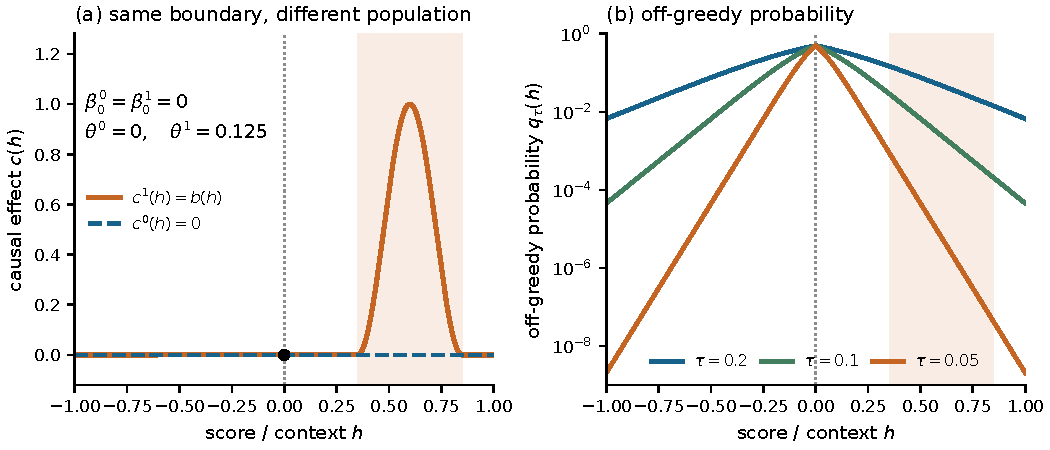
\includegraphics[width=\textwidth]{figs/fig1_mechanism.pdf}
\caption{Construction behind Theorem~\ref{thm:separation} (Model I is $\mu^0$,
Model II is $\mu^t$), with $H\sim U(-1,1)$, $g(h)=|h|$, $u_1=0.35$, $u_2=0.85$ and
$t=1$. Left: effect functions. Both boundary effects are zero; the population
effects are $0$ and $0.125$. Right: probability of the unpreferred action at three
temperatures. The models differ only in the shaded region.}
\label{fig:separation}
\end{figure}

The paper makes three contributions. Theorems~\ref{thm:boundary}
and~\ref{thm:separation} establish the separation in a model with Gaussian outcomes
and globally Lipschitz mean functions. With $\tau_n=n^{-\zeta}$ and
$\zeta\in(1/2,1)$, Wald intervals for the boundary effect are uniformly valid and
$R_n\to0$, while uniformly consistent estimation of the population effect requires
$\sup R_n\to\infty$. Theorem~\ref{thm:info} is an information--exploration
inequality for all estimators and adaptive designs when the mean functions are only
bounded, and Proposition~\ref{prop:achieve} shows that a gap-based design attains its
order. Section~\ref{sec:temperature} turns to design. A single common temperature is
costly for the population effect; uniform mixing, context-specific temperatures and
some temperature mixtures are not.

Throughout, each unit receives one decision, contexts are independent and the
assignment probabilities are known. The score and the preferred action are fixed
functions of the context. By ``adaptive'' we mean sharpening, or designs that use
past data, and not a bandit that learns from outcomes which action is better. Other
limitations are collected in Section~\ref{sec:discussion}.

The paper is organized as follows. Section~\ref{sec:setup} sets out the model and
Section~\ref{sec:brief} previews the results. Sections~\ref{sec:boundary},
\ref{sec:population} and~\ref{sec:separation} treat the boundary effect, the
population effect and the separation. Section~\ref{sec:temperature} discusses
temperature as a design choice, Section~\ref{sec:sims} reports simulations and
Section~\ref{sec:discussion} concludes. Proofs are in the appendix.

\paragraph{Related work.}
The boundary result is closest to work that uses algorithmic or mechanism-based
assignment as a source of local randomization. Lee~\cite{lee2008randomized} reads
regression discontinuity as local randomization. Abdulkadiro\u{g}lu et
al.~\cite{abdulkadiroglu2017research,abdulkadiroglu2022breaking} use propensity
scores induced by school-assignment mechanisms, including local scores near
tie-breaking cutoffs, and Narita and Yata~\cite{narita2021algorithm} show that
overlap-type weights built from an approximate propensity score of a known algorithm
converge to a boundary estimand. In their work the analyst chooses how much to
smooth. Here the system's temperature plays that role, and we keep track of the
exploration loss that comes with it. Eckles et al.~\cite{eckles2020noise} exploit
known assignment noise of fixed scale at a cutoff. Overlap weights go back to Li,
Morgan and Zaslavsky~\cite{li2018balancing}, and Humphreys~\cite{humphreys2025bounds}
shows that fixed-effects regression weights stratum effects by $p_j(1-p_j)$; under a
sharpening policy almost all of that weight sits at the boundary.

The trade-off between reward and estimation has mostly been studied for bandits
without contexts~\cite{erraqabi2017trading,simchilevi2023multi}, where the
guarantees concern particular algorithms. Liang and Bojinov~\cite{liang2023mixture}
are closest to our design conclusions. They mix any bandit algorithm with a
Bernoulli design whose weight decays more slowly than $t^{-1/4}$ and obtain
anytime-valid confidence sequences for the average effect. Their setting has no
contexts and no cost for the Bernoulli assignments; we charge each departure from
the deployer's preferred action by its value gap, and Theorem~\ref{thm:info} bounds from below
the loss that any design must incur to learn the population effect uniformly.
Hadad et al.~\cite{hadad2021confidence} build confidence
intervals for policy values from bandit data when assignment probabilities decay no faster
than a polynomial rate. Under a sharpening policy the probabilities decay exponentially in
$|\Delta|/\tau$ away from the boundary, and our boundary estimator targets
$\beta_0$ rather than a policy value. Adaptive designs have also been proposed for
efficient estimation of average effects~\cite{kato2020efficient}, for policy
choice~\cite{kasy2021adaptive} and for applications in political
science~\cite{offerwestort2021adaptive}; in those designs assignment serves
estimation or choice, whereas here it is fixed by the deployer's objective.
Conservative bandits~\cite{wu2016conservative} keep cumulative reward above that of a
baseline policy, and Wan, Kveton and Song~\cite{wan2022safe} optimize exploration for
policy evaluation under a value constraint; both measure cost against a baseline, as
we do, but their guarantees concern the regret or evaluation error of the proposed
algorithms. Tucker and Joachims~\cite{tucker2023variance} and Douglas, Persson and
Provost~\cite{douglas2026logging} choose logging policies to reduce the variance of
off-policy estimates, and Koppel et al.~\cite{koppel2025explore} balance regret
against the quality of average-effect estimates in contextual bandits. The allocation $q\propto g^{-1/2}$ is optimum
stratified allocation with costs~\cite{cochran1977sampling} and appears for factorial
experiments in~\cite{ravichandran2024optimal}; what we add is that its constant bounds
every estimator and adaptive design. Li and Imai~\cite{li2024neyman} compare ways of
evaluating an individualized rule without charging for departures from it, and
Cesa-Bianchi et al.~\cite{cesabianchi2017boltzmann} show that Boltzmann exploration
with one schedule can fail for regret. Theorem~\ref{thm:common} is an analogue for
estimation.

The lower bounds draw on off-policy evaluation~\cite{li2015toward,wang2017optimal,mou2023off}
and on limited overlap and trimming
\cite{khan2010irregular,crump2009dealing,rothe2017robust,hong2020inference,ma2020robust},
in particular the irregular identification of Khan and Tamer~\cite{khan2010irregular}.
Ring and Schomaker~\cite{ring2026diagnostic} use positivity diagnostics to choose
alternative estimands, and Khan, Saveski and Ugander~\cite{khan2024off} bound effects
without overlap by assuming smoothness, the kind of extrapolation our lower bounds
rule out. For generative treatments, Athey, Imbens and Ji~\cite{athey2026stochastic}
identify effects of content features from stochastic algorithms, Fresh and
Shin~\cite{fresh2026conversation} classify conversational estimands, and Imai and
Nakamura~\cite{imai2026causal,nakamura2026dynamic} study effects of realized text. We
stay at the level of strategy assignment and hold the generator fixed.

%=============================================================================
\section{Setup}\label{sec:setup}

\paragraph{Treatments.} Units $i=1,\dots,n$ arrive with contexts $H_i\sim F$.
The system chooses a strategy $A_i\in\{0,1\}$ and produces a message
$M_i\sim G(\cdot\mid A_i,H_i)$ from a fixed generation kernel $G$, which includes
token-level sampling settings; the outcome is $Y_i$. The treatment is the
assignment of the strategy with $G$ held fixed, so potential outcomes $Y_i(a)$
include the randomness of the message
\cite{munoz2012population,young2014identification}; changing $G$ changes the
treatment. We assume:
\begin{enumerate}[label=(C\arabic*),leftmargin=3em,itemsep=1pt]
\item \emph{consistency}: $Y_i=Y_i(A_i)$;
\item \emph{independent units}: $(H_i,Y_i(0),Y_i(1))$ are independent and
identically distributed across $i$, with no interference;
\item \emph{sequential ignorability with known probabilities}: $A_i$ is independent
of $(Y_i(0),Y_i(1))$ given $(H_i,\mathcal F_{i-1})$, where $\mathcal F_{i-1}$ is
the data of units $1,\dots,i-1$, and $\Prob(A_i=1\mid H_i,\mathcal F_{i-1})$ is known.
\end{enumerate}
Then the law of $Y_i$ given $(A_i=a,H_i=h,\mathcal F_{i-1})$ is that of $Y(a)$
given $H=h$, so statements about conditional outcome laws are statements about
potential outcomes.

\paragraph{Deployer.} The deployer has a score gap $\Delta(h)=s_1(h)-s_0(h)$
from its own objective, a preferred (greedy) action $a^*(h)=\mathbf 1\{\Delta(h)>0\}$,
and an operational value gap $g(h)\ge0$, the value its objective loses by choosing
$\bar a(h)=1-a^*(h)$. We write $g=\phi(|\Delta|)$ when the gap is a function of the
score. The score and the preferred action are fixed functions of the context.

\paragraph{Running example.} A conversational system chooses between presenting
evidence ($A=1$) and asking a question ($A=0$). A reward model scores both
strategies given the conversation so far, $H$; $\Delta(H)$ is the score difference,
and the system logs the probability with which it chose evidence. The operational
gap $g(H)$ is the loss in the deployer's objective, for example predicted
engagement, from using the lower-scoring strategy. The outcome $Y$ is the person's
attitude after the conversation, measured separately and not used by the policy.

\paragraph{Probabilities and designs.} We write
\[
e(h)=\Prob(A=1\mid H=h),\qquad q(h)=\Prob(A\neq a^*(h)\mid H=h)
\]
for the probability of action $1$ and of the non-preferred action. A design is
non-adaptive if these probabilities do not depend on past data. A \emph{common
temperature} design uses one deterministic $\tau=\tau_n$ and
\[
e_\tau(h)=\sgm(\Delta(h)/\tau),\qquad q_\tau(h)=\sgm(-|\Delta(h)|/\tau),
\qquad \sgm(x)=1/(1+\exp(-x)).
\]

\paragraph{Exploration loss.} The expected cumulative operational loss is
\begin{equation}\label{eq:loss-definition}
 R_n=\E\left[\sum_{i=1}^n g(H_i)\mathbf 1\{A_i=\bar a(H_i)\}\right],
\end{equation}
and $R_n=n\E[g(H)q(H)]$ for non-adaptive designs. Under adaptive designs $R_n$
may depend on the outcome law through past observations.

\paragraph{Estimands.} Let $\mu_a(h)=\E[Y(a)\mid H=h]$ and $c=\mu_1-\mu_0$. The
population average effect is $\theta=\E[c(H)]$. With a one-dimensional score
$\Delta(h)=h$ the boundary effect is $\beta_0=c(0)$. For a given temperature, the
overlap-weighted effect
$\beta_{\ov,\tau}=\E[\omega_\tau(H)c(H)]/\E[\omega_\tau(H)]$, with
$\omega_\tau=e_\tau(1-e_\tau)$ \cite{li2018balancing}, is an intermediate target.

%=============================================================================
\section{The results in brief}\label{sec:brief}

Take $\Delta(h)=h$, Gaussian outcomes with variance $\sigma^2$, and mean functions
bounded by $B$ and $L$-Lipschitz; call this model $\Mlip$. Suppose the logs come from
one common temperature $\tau_n=n^{-\zeta}$ with $\zeta\in(1/2,1)$ and that the
operational gap vanishes linearly at the boundary. Then:
\begin{enumerate}[label=(\roman*),leftmargin=2em,itemsep=2pt]
\item the Wald interval for the boundary effect is asymptotically valid uniformly
over $\Mlip$, and $R_n\to0$ (Theorems~\ref{thm:boundary} and~\ref{thm:separation});
\item $\Mlip$ contains two outcome laws with the same boundary effect and different
population effects that differ only for the non-preferred action, in a region where
the gap is bounded below. Once $R_n\to0$, no estimator is consistent for the
population effect at both, and uniformly consistent estimation over $\Mlip$ requires
divergent worst-case loss (Theorem~\ref{thm:separation});
\item if the mean functions are only bounded, precision $\delta$ for the population
effect requires worst-case loss of order at least $(\E\sqrt g)^2/\delta^2$ as
$\delta\to0$, whatever the value of $n$ (Theorem~\ref{thm:info}).
\end{enumerate}
Figure~\ref{fig:map} shows what this looks like in the simulation design of
Section~\ref{sec:sims}. Under one common temperature, the Horvitz--Thompson estimator
of the population effect reaches root mean squared error $\figDelta$ only where the
loss is at least about $\figPopMinLoss$ on the plotted grid. The boundary effect
reaches the same precision with loss $\figBndMinLoss$ at the edge of the grid, and
with less at larger $n$. Panel (a) describes a single estimator; the lower bounds for
all estimators are Theorems~\ref{thm:info} and~\ref{thm:separation}.

\begin{figure}[tbp]
\centering
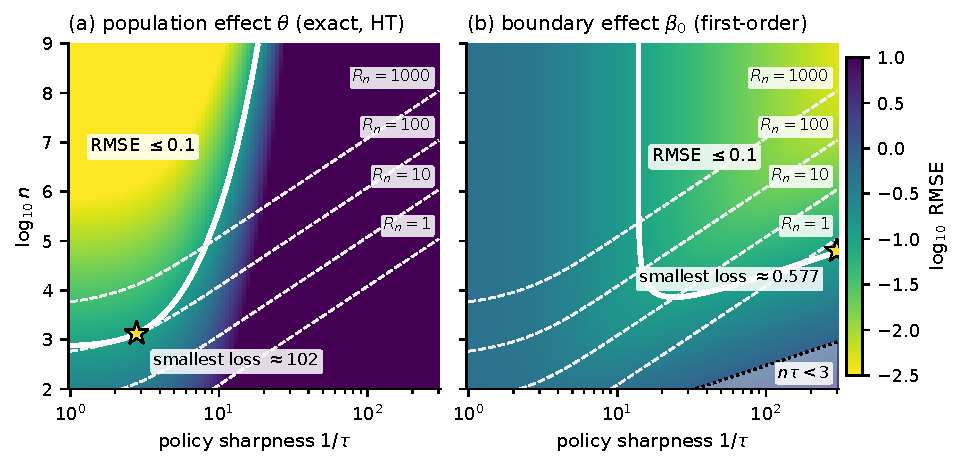
\includegraphics[width=\textwidth]{figs/fig2_separation_map.pdf}
\caption{Root mean squared error ($\log_{10}$ scale) under one common temperature,
in the design of Section~\ref{sec:sims}. (a) Exact value for the Horvitz--Thompson
estimator of $\theta$. (b) First-order approximation
$\{(\beta_{\ov,\tau}-\beta_0)^2+s_n^2/n\}^{1/2}$ for the estimator of
Theorem~\ref{thm:boundary}, checked by simulation in Section~\ref{sec:sims}. White
curves enclose error at most $\figDelta$, dashed curves are levels of $R_n$, and stars
mark the smallest loss reaching that precision on the grid. The approximation was
not checked in the shaded region $n\tau<3$.}
\label{fig:map}
\end{figure}

%=============================================================================
\section{Boundary effects at vanishing exploration loss}\label{sec:boundary}

\begin{assumption}[Boundary model]\label{ass:D}
$\Delta(h)=h$, $a^*(h)=\mathbf 1\{h>0\}$, and
\begin{enumerate}[label=(D\arabic*),leftmargin=3em,itemsep=1pt]
\item $H$ has a density $f\le\bar f$, continuous at $0$, with $f(0)>0$;
\item $|\mu_a|\le B$, and $\mu_a$ is $L$-Lipschitz on $[-u_0,u_0]$;
\item $\sigma_a^2(h)=\Var(Y\mid A=a,H=h)$ is continuous at $0$ with
$\sigma_1^2(0)+\sigma_0^2(0)>0$, and $\E[Y^4\mid A,H]\le M_4$;
\item $\Prob(A=1\mid H=h)=\sgm(h/\tau_n)$ with $\tau_n\to0$, known;
\item $g=\phi(|h|)\le\bar G$ with $\phi(u)\le\bar\kappa u$ on $[0,u_0]$; in the
strong form $\phi'(0)=\kappa>0$.
\end{enumerate}
\end{assumption}

With $e_i=e_{\tau_n}(H_i)$, define
\begin{align}
 w_{1i}&=A_i(1-e_i), & w_{0i}&=(1-A_i)e_i,\nonumber\\
 \hat D_a&=\frac1n\sum_{i=1}^n w_{ai}, &
 \hat m_a&=\frac{\sum_{i=1}^n w_{ai}Y_i}{\sum_{i=1}^n w_{ai}},
 &\hat\beta&=\hat m_1-\hat m_0,\label{eq:boundary-estimator}\\
 \hat\psi_i&=\frac{w_{1i}(Y_i-\hat m_1)}{\hat D_1}
             -\frac{w_{0i}(Y_i-\hat m_0)}{\hat D_0}, &
 \hat s^2&=\frac1n\sum_{i=1}^n\hat\psi_i^2. \label{eq:boundary-se}
\end{align}
If either weight sum is zero, set $\hat\beta=\hat s^2=0$ and report the interval
$\mathbb R$; this event has probability tending to zero when $n\tau_n\to\infty$.
Write $m_\tau=\E[\omega_\tau(H)]$, $\bar\mu_a=\E[\omega_\tau(H)\mu_a(H)]/m_\tau$,
\[
\xi=\frac{w_1(Y-\bar\mu_1)-w_0(Y-\bar\mu_0)}{m_\tau},\qquad s_n^2=\Var(\xi),
\]
so that $\bar\mu_1-\bar\mu_0=\beta_{\ov,\tau}$ and $\xi$ is the linearization of
$\hat\beta-\beta_{\ov,\tau}$.

\begin{theorem}[Boundary inference]\label{thm:boundary}
Under Assumption~\ref{ass:D}, if $n\tau_n\to\infty$:
\begin{enumerate}[label=(\roman*),leftmargin=2em,itemsep=1pt]
\item $(\hat\beta-\beta_{\ov,\tau_n})/(s_n/\sqrt n)\Rightarrow N(0,1)$, and
$s_n^2=\{\sigma_1^2(0)+\sigma_0^2(0)\}/\{2\tau_nf(0)\}\,(1+o(1))$;
\item $|\beta_{\ov,\tau_n}-\beta_0|\le C\tau_n$ for large $n$, for every
$C>4\log2\,L\bar f/f(0)$;
\item $\hat s^2/s_n^2\to1$ in probability;
\item if also $n\tau_n^3\to0$, the Wald interval $\hat\beta\pm
z_{1-\eta/2}\hat s/\sqrt n$ has asymptotic coverage $1-\eta$ for $\beta_0$;
\item $R_n=n\E[g(H)q_{\tau_n}(H)]\le n\tau_n^2\bar\kappa\bar f\pi^2/6+n\bar G\exp(-u_0/\tau_n)$, and in
the strong form $R_n=n\tau_n^2\kappa f(0)\pi^2/6\,(1+o(1))$.
\end{enumerate}
In particular, for $\tau_n=n^{-\zeta}$ with $\zeta\in(1/2,1)$, the interval in
(iv) is asymptotically valid and $R_n\to0$.
\end{theorem}

The three rate conditions say that the boundary sample grows ($n\tau_n\to\infty$,
$\zeta<1$), that the bias is small next to the standard error ($n\tau_n^3\to0$,
$\zeta>1/3$) and that the loss vanishes ($n\tau_n^2\to0$, $\zeta>1/2$). At
$\zeta=1/2$ the interval is still valid and the loss stays bounded. The error is
$O_p((n\tau_n)^{-1/2}+\tau_n)$; optimality of this rate is not established here.
A smoother effect helps only with more structure. If $c$ is $C^{1,1}$ and $f$ is
Lipschitz near zero, the bias is $O(\tau^2)$ and (iv) needs only $n\tau_n^5\to0$, but
an effect equal to $1+|h|^{3/2}$ near zero, which is differentiable, still has bias
of order $\tau^{3/2}$. Proofs are in Appendix~\ref{app:boundary}.

Exploration continues even as the loss vanishes. The expected number of non-preferred
actions, $n\E[q_{\tau_n}(H)]=2\log2\,f(0)\,n\tau_n(1+o(1))$, grows with $n$. The loss
goes to zero because these actions happen ever closer to the boundary, where they
cost little. How much they cost there depends on the shape of the gap.

\begin{proposition}[Shape of the operational gap]\label{prop:gapshape}
Let (D1) and (D4) hold and $g=\phi(|h|)\le\bar G$.
\begin{enumerate}[label=(\alph*),leftmargin=2em,itemsep=1pt]
\item If $\phi(u)\le\bar\kappa u^p$ on $[0,u_0]$ for some $p>0$, then
$R_n\le 2\bar\kappa\bar f C_p\,n\tau_n^{p+1}+n\bar G\exp(-u_0/\tau_n)$ with
$C_p=\int_0^\infty v^p\sgm(-v)\,dv<\infty$. Under the other conditions of
Theorem~\ref{thm:boundary}, $\tau_n=n^{-\zeta}$ with
$\max\{1/3,1/(p+1)\}<\zeta<1$ gives a valid interval for $\beta_0$ and $R_n\to0$.
\item If $\phi(u)\ge\lambda_0>0$ for $u\in(0,u_0]$, then
$R_n\ge2\log2\,\lambda_0f(0)\,n\tau_n(1+o(1))$, which diverges whenever
$n\tau_n\to\infty$, the condition under which Theorem~\ref{thm:boundary} applies.
\end{enumerate}
\end{proposition}

Part (b) applies to any cost charged per deviation regardless of context, such as a
human review or a payment. With such costs the loss of boundary inference under a
common temperature diverges too, and the contrast of Section~\ref{sec:separation}
disappears. Part (b) concerns this design only; it does not compare the least
possible costs of the two targets. The proof is in Appendix~\ref{app:boundary}.

%=============================================================================
\section{Population effects require paid exploration}\label{sec:population}

Fix $B>0$ and $\sigma>0$. Let $\M(B,\sigma)$ be the model in which
$Y\mid A=a,H=h$ is $N(\mu_a(h),\sigma^2)$ and $\mu_0,\mu_1$ are \emph{any}
measurable functions bounded by $B$. Nothing in this model links effects near the
boundary to effects elsewhere.

\begin{theorem}[Information--exploration inequality]\label{thm:info}
Let $S_1,\dots,S_J$ be disjoint sets with $f_j=F(S_j)>0$, each contained in
$\{a^*=0\}$ or in $\{a^*=1\}$, and $g_j=\essinf_{S_j}g$. For every design,
adaptive or not, and every estimator $\hat\theta$,
\begin{equation}\label{eq:info}
\sup_{\M(B,\sigma)}\E(\hat\theta-\theta)^2\cdot
\Big(\sup_{\M(B,\sigma)}R_n+\frac{\sigma^2\pi^2}{B^2}\sum_j g_j\Big)
\;\ge\;\sigma^2\Big(\sum_jf_j\sqrt{g_j}\Big)^2 .
\end{equation}
Consequently, if $F(g\ge\gamma)>0$ for some $\gamma>0$, uniform consistency
requires $\sup R_n\to\infty$; and if $\sup\E(\hat\theta-\theta)^2\le\delta_n^2\to0$,
then $\liminf_n\delta_n^2\sup R_n\ge\sigma^2(\E\sqrt{g(H)})^2$.
\end{theorem}

The sample size does not appear in \eqref{eq:info}, so the lower bound on the
exploration loss needed for a given precision does not decrease as the deployment
grows. At a fixed precision $\delta$, the
inequality gives
$\sup R_n\ge\sigma^2(\sum_jf_j\sqrt{g_j})^2/\delta^2-\sigma^2\pi^2\sum_jg_j/B^2$.
The best partition gives at most $\sigma^2(\E\sqrt g)^2/\delta^2$, and that constant
is reached only as $\delta\to0$. At $R_n=0$ and $\sum_jg_j>0$ the bound is the finite
floor $B^2(\sum_jf_j\sqrt{g_j})^2/(\pi^2\sum_jg_j)$, as it should be, since a
constant estimator has bounded error.

\begin{proposition}[Achievability]\label{prop:achieve}
Suppose $0<\E\sqrt g<\infty$, $\delta_n>0$ and $n\delta_n^2\to\infty$. Write
$C=\sigma^2+B^2$. For $n\delta_n^2>4C$, define
\begin{equation}\label{eq:allocation}
 c_n=\frac{\E\sqrt g}{n\delta_n^2/C-4},\qquad
 q_n(h)=\begin{cases}
 \min\{1/2,c_n/\sqrt{g(h)}\},&g(h)>0,\\
 1/2,&g(h)=0,
 \end{cases}
\end{equation}
and let $e_n(h)$ be the corresponding probability of action $1$. The
Horvitz--Thompson estimator
\begin{equation}\label{eq:ht}
 \hat\theta_{\rm HT}=\frac1n\sum_{i=1}^n
 \left\{\frac{A_iY_i}{e_n(H_i)}-
 \frac{(1-A_i)Y_i}{1-e_n(H_i)}\right\}
\end{equation}
has $\sup_{\M(B,\sigma)}\E(\hat\theta_{\rm HT}-\theta)^2\le\delta_n^2$ and
$R_n\le Cn(\E\sqrt g)^2/(n\delta_n^2-4C)=C(\E\sqrt g)^2\delta_n^{-2}(1+o(1))$.
If also $\E[g]<\infty$, uniform mixing with $q\equiv C/(n\delta_n^2-2C)$, for
$n\delta_n^2\ge4C$, has the same uniform risk guarantee and
$R_n=Cn\E[g]/(n\delta_n^2-2C)=C\E[g]\delta_n^{-2}(1+o(1))$.
\end{proposition}

The lower bound and the attainable loss share the order $\delta^{-2}$ and the
functional $(\E\sqrt g)^2$. Their constants are $\sigma^2$ and $\sigma^2+B^2$, which
can be far apart when $B^2\gg\sigma^2$, and we have not found the optimal one. Proofs
are in Appendix~\ref{app:population}.

%=============================================================================
\section{The separation in one model}\label{sec:separation}

Theorem~\ref{thm:info} is proved in $\M(B,\sigma)$, which places no restriction
away from the boundary. A lower bound in a large model says nothing about a smaller
one, so we now work with a single model that is smooth everywhere. Fix $F$ satisfying
(D1), $g=\phi(|h|)$ satisfying (D5), and $B,L,\sigma>0$. Let $\Mlip$ be the set of
outcome laws with $Y\mid A=a,H=h\sim N(\mu_a(h),\sigma^2)$ and $\mu_0,\mu_1$ bounded
by $B$ and $L$-Lipschitz on $\mathbb R$. Every member of $\Mlip$ satisfies (D2)
and (D3).

\begin{assumption}\label{ass:SA}
There are $0<u_1<u_2$ with $F([u_1,u_2])>0$ and
$\gamma:=\essinf_{h\in[u_1,u_2]}g(h)>0$.
\end{assumption}

\begin{theorem}[Separation]\label{thm:separation}
Under Assumption~\ref{ass:SA}, let
$b(h)=\sin^2(\pi(h-u_1)/(u_2-u_1))\mathbf 1\{u_1\le h\le u_2\}$,
$t_{\max}=\min\{B,L(u_2-u_1)/\pi\}$, and for $|t|\le t_{\max}$ let $\mu^t$ have
$\mu^t_1\equiv0$ and $\mu^t_0=-tb$. Then $\mu^t\in\Mlip$, all $\mu^t$ coincide on
$(-\infty,u_1]$, $\beta_0(\mu^t)=0$ and $\theta(\mu^t)=t\E[b(H)]$.
\begin{enumerate}[label=(S\arabic*),leftmargin=3em,itemsep=2pt]
\item Under the common-temperature design $\tau_n=n^{-\zeta}$, $\zeta\in(1/2,1)$,
$R_n\to0$ and
$\sup_{\mu\in\Mlip}\big|P_\mu\{\beta_0(\mu)\in\hat\beta\pm z_{1-\eta/2}\hat s/\sqrt n\}-(1-\eta)\big|\to0$.
\item For every design and every $t$,
$\TV(P^n_{\mu^0},P^n_{\mu^t})\le R_n(\mu^0)/\gamma$. Hence if $R_n(\mu^0)\to0$,
for every $t_1\in(0,t_{\max}]$ and every estimator,
$\max_{t\in\{0,t_1\}}P_{\mu^t}(|\hat\theta_n-\theta(\mu^t)|\ge t_1\E[b]/2)\ge
(1-R_n(\mu^0)/\gamma)/2\to1/2$.
\item For every design and every estimator,
\[
\sup_{\Mlip}\E(\hat\theta-\theta)^2\ge\frac{(\E[b])^2}{\sup_{\Mlip}R_n/(\sigma^2\gamma)+\pi^2/t_{\max}^2}.
\]
\end{enumerate}
\end{theorem}

Both halves are now uniform over the same model. (S1) gives boundary intervals with
uniformly correct coverage, (S3) shows that uniform consistency for the population
effect needs unbounded worst-case loss, and (S2) makes the same point for two fixed
members. Since $\theta\in[-2B,2B]$, an estimator can be clipped to that interval, so
consistency in probability and in mean square are equivalent here. Whether the
constant of Theorem~\ref{thm:info} holds in $\Mlip$ is open. In submodels where
boundary data identify $\theta$ the perturbation family is not available, and (S2)
and (S3) do not apply. Proofs are in Appendix~\ref{app:separation}.

%=============================================================================
\section{Temperature as an exploration device}\label{sec:temperature}

\begin{theorem}[One common temperature]\label{thm:common}
Consider common-temperature designs with one deterministic $\tau_n$ per $n$.
Assume $g=\phi(|\Delta|)$ with $\E[g]<\infty$; $|\Delta(H)|$ has a density at least
$f_{\min}>0$ on $[0,v_0]$; $\phi(u)\ge\underline\kappa u$ on $[0,v_0]$; and
$D_{\max}=\esssup|\Delta(H)|<\infty$. Fix $\epsilon\in(0,D_{\max})$ and let
$\nu_\epsilon=\max_j\Prob(|\Delta(H)|\ge D_{\max}-\epsilon,\ a^*(H)=j)$, which is
positive. If an estimator has $\sup_{\M(B,\sigma)}\E(\hat\theta-\theta)^2\le\delta_n^2$
with $\delta_n^2\le\nu_\epsilon^2B^2/(2\pi^2)$ and $2n\delta_n^2>\nu_\epsilon\sigma^2$,
then
\[
R_n\ \ge\ \underline\kappa f_{\min}c_*\,n\min\Big\{v_0^2,\ \frac{(D_{\max}-\epsilon)^2}{\log^2\{2n\delta_n^2/(\nu_\epsilon\sigma^2)\}}\Big\},
\qquad c_*=\int_0^1v\,\sgm(-v)\,dv .
\]
\end{theorem}

The precision $\delta_n$ may be fixed. For fixed $\delta$ with
$\delta^2\le\nu_\epsilon^2B^2/(2\pi^2)$, a common temperature needs loss of order at
least $n/\log^2n$, while Proposition~\ref{prop:achieve} reaches the same precision with
loss bounded in $n$. Some condition on $\delta$ is needed: for $\delta\ge2B$ the
estimator that always returns zero meets the target without exploring. The theorem
holds in $\M(B,\sigma)$; with a correctly specified parametric outcome model, a
model-based estimator can do better. A common temperature explores most near the
boundary, and so does the optimal design, so the location of exploration is not the
issue. The issue is that the probability of the non-preferred action decays
exponentially in $|\Delta|$. Confident contexts are then almost never explored unless
the temperature is raised everywhere, which increases the loss incurred in contexts
near the boundary.

\begin{remark}[Mixtures of temperatures]\label{rem:mixture}
Theorem~\ref{thm:common} does not extend to random mixtures of finite temperatures.
With $|\Delta|=|H|$, $H\sim U(-1,1)$ and $g=|H|$, let $r(u)=\sgm(-u)$ be the
non-preferred probability at temperature $1$, and mix temperature $1$ with weight
$w_n=\E[1/r(|H|)]/\{n\delta^2/(\sigma^2+B^2)-2\}$ and temperature $1/n$ otherwise.
The Horvitz--Thompson estimator then has uniform mean squared error at most
$\delta^2$ over $\M(B,\sigma)$, and the loss is at most
$(\sigma^2+B^2)\E[1/r]\E[|H|r]/\delta^2+O(1/n)$, bounded in $n$; at $\delta=0.1$ the
factor $\E[1/r]\E[|H|r]/\delta^2$ equals \mixtureCost{}. What is costly is one
temperature shared by all contexts.
\end{remark}

\begin{proposition}[Context temperatures]\label{prop:ctx}
For $\Delta(h)\neq0$ and $q(h)\in(0,1/2)$, the context temperature
$\tau(h)=|\Delta(h)|/\log\{(1-q(h))/q(h)\}$ gives non-preferred probability $q(h)$;
$q(h)=1/2$ requires $\tau(h)=\infty$, and on $\{\Delta=0\}$ every temperature gives
$q=1/2$. If $g=\phi(|\Delta|)$ with $\phi(0)=0$, the design $q_n$ of
Proposition~\ref{prop:achieve} is implementable with temperatures in $(0,\infty]$,
and for each $h$ with $\Delta(h)\neq0$ and $g(h)>0$, $\tau_n(h)\log(1/c_n)\to|\Delta(h)|$.
\end{proposition}

The limit holds for each $h$. Where the cap binds, for example $0<|h|\le4c_n^2$ when
$g(h)=|h|$, the temperature is $\tau=\infty$. If the gap is known only up to a
multiplicative error, Lemma~\ref{lem:robust} in Appendix~\ref{app:temperature} bounds
the extra cost of allocating by the wrong gap. Proofs are in
Appendix~\ref{app:temperature}.

%=============================================================================
\section{Simulations}\label{sec:sims}

The simulations use $H\sim U(-1,1)$, $\Delta(h)=h$, $g(h)=|h|$, $\mu_0(h)=h$,
$c(h)=1+|h|$ (population effect $1.5$, boundary effect $1$) and $N(0,1)$ noise.
Code, seeds and result files are in the repository cited in the data availability
statement.

\paragraph{Exploration designs.} To compare allocations we hold fixed the
sparse-exploration criterion $V_{\rm sp}(q)=\sigma^2\E[1/q]/n$. This is a criterion for
allocation, not the mean squared error of a particular estimator. At $n=10^5$ and
$V_{\rm sp}=0.01$ the exploration loss is \costUniform{} for uniform mixing,
\costOptimal{} for the gap-based design $q\propto g^{-1/2}$ and \costCommon{} for a
common temperature ($\tau=\costCommonTau$), about \costRatioCommonUniform{} times the
loss of uniform mixing (Figure~\ref{fig:costs}; Figure~\ref{fig:costs-small} in
Appendix~\ref{app:figures} repeats this at $V_{\rm sp}=0.03^2$). The gap-based design
here is calibrated to $V_{\rm sp}$ and capped at $1/2$, rather than using the $c_n$ of
Proposition~\ref{prop:achieve}. Table~\ref{tab:designs} runs the augmented
inverse-propensity estimator on common random numbers, with a working model linear in
$(1,H,|H|)$ in each arm, which is correct for this design. Implementing the gap-based
design through context temperatures gives identical rows. Because $V_{\rm sp}$ is
fixed, the expected number of non-preferred actions stays bounded for uniform mixing
and the gap-based design, so the nominal coverage of their Wald intervals has no
asymptotic justification as $n$ grows. In a two-context example with masses
$(0.5,0.5)$, gaps $(0.2,1)$, $\sigma=1$, $B=5$ and $\delta=0.1$, the bound
\eqref{eq:info} equals \finiteBound{}, against an asymptotic constant of
\finiteConstant{}, and the common-temperature loss grows locally like $n$ to the power
\finiteSlope{}, close to the predicted $1-\Delta_{\min}/\Delta_{\max}=0.8$.

\begin{figure}[tbp]
\centering
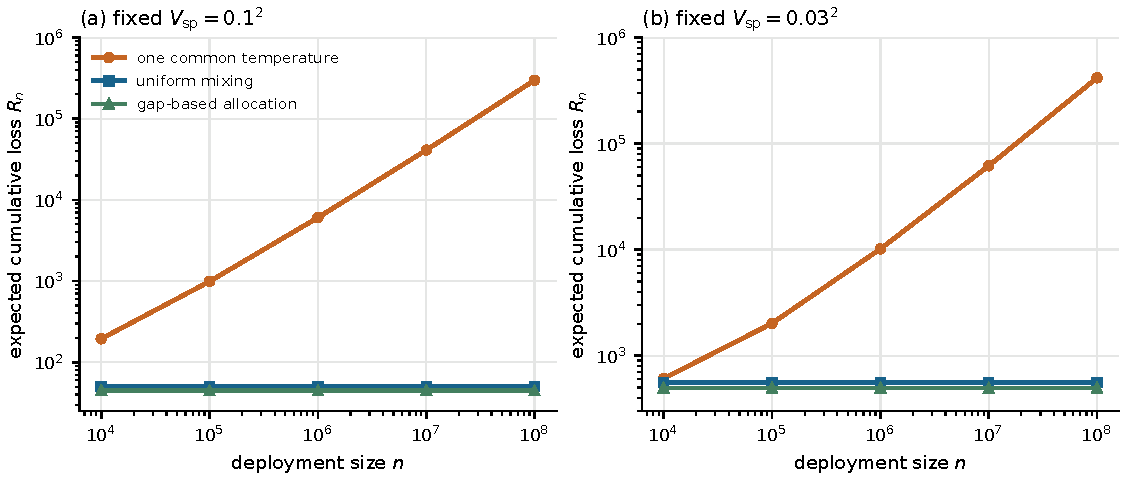
\includegraphics[width=0.66\textwidth]{figs/fig3_exploration_costs.pdf}
\caption{Exploration loss against deployment size, in closed form, with the
sparse-exploration criterion fixed at $V_{\rm sp}=0.1^2$.}
\label{fig:costs}
\end{figure}

\begin{table}[tbp]
\centering\small
\tabDesigns
\caption{Exploration designs at $n=10^5$, 400 replications with common random
numbers. Coverage is of the population effect by Wald intervals; MCSE uses the
observed coverage. ``Explored'' is the mean number of non-preferred actions.}
\label{tab:designs}
\end{table}

\paragraph{Boundary inference.} Table~\ref{tab:boundary} reports the estimator of
Theorem~\ref{thm:boundary}. The exploration loss agrees with the constant in
Theorem~\ref{thm:boundary}(v). With $\zeta=0.6$ coverage is close to nominal: at
$n=10^6$, 5,000 replications give \covFiveK{} (MCSE \covFiveKmcse), and the estimated
standard error is \covFiveKseRatio{} times the Monte Carlo standard deviation. When
the boundary sample is very small the interval under-covers, with \covSmallNtau{} at
$n\tau_n\approx\smallNtau$. We also checked the first-order approximation used in
Figure~\ref{fig:map}(b), with \foReps{} replications per setting and undefined
estimates set to zero. The ratio of Monte Carlo to approximate root mean squared error
lies between \foRatioMin{} and \foRatioMax{} in the \foCells{} settings with
$n\tau\ge3$. At $n\tau=\foNtauTiny$, where \foUndefPct\% of the estimates were
undefined, it is \foRatioTiny{}.

\begin{table}[tbp]
\centering\small
\tabBoundary
\caption{Boundary inference under common temperature $\tau_n=n^{-\zeta}$. Coverage
is of $\beta_0=c(0)$. Loss is the Monte Carlo mean with the
Theorem~\ref{thm:boundary}(v) constant in parentheses. The last row is a separate
5,000-replication run.}
\label{tab:boundary}
\end{table}

\paragraph{Temperature sweep.} Figure~\ref{fig:sweep} fixes $n=\curveN$ and sharpens
a common temperature, with \curveReps{} replications per temperature. Coverage of the
population effect falls from \curvePopCovLo{} at $1/\tau=1$ to \curvePopCovHi{} for
the Horvitz--Thompson estimator and \curveAipwCovHi{} for the augmented estimator at
$1/\tau=\curveInvTauMax$. Coverage of the boundary effect rises from \curveBndCovLo{}
to \curveBndCovHi{}. At $1/\tau=1$ the interval is centred on $\beta_{\ov,\tau}$, which
is \curveBndBiasLo{} away from $\beta_0$, and the gap closes as $\tau$ falls. Meanwhile
the exploration loss drops from \curveLossLo{} to \curveLossHi{}. Over this range
$n\tau$ stays above \curveNtauMin{}; pushing the temperature lower at fixed $n$ would
eventually break the boundary interval as well (Table~\ref{tab:boundary}). Once the
policy is sharp, Monte Carlo understates the error of the Horvitz--Thompson estimator.
At $1/\tau=\curveInvTauMax$ its Monte Carlo root mean squared error is
\curveHtMcRmseHi{}, but its exact standard deviation is of order
$10^{\curveHtExactSdHiExp}$, driven by rare and very large terms that the replications
never draw (Figure~\ref{fig:sweep-error} in Appendix~\ref{app:figures}).

\begin{figure}[tbp]
\centering
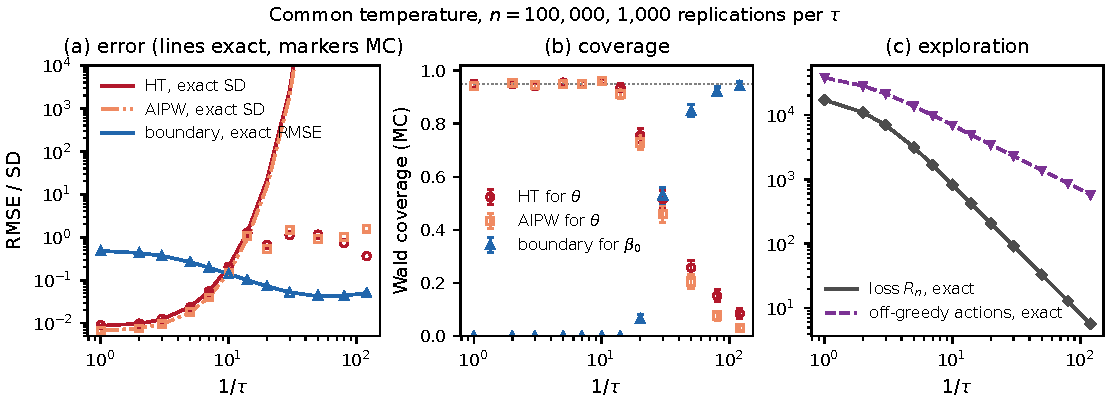
\includegraphics[width=\textwidth]{figs/fig4_temperature_sweep.pdf}
\caption{Sharpening a common temperature at $n=\curveN$. (a) Coverage of Wald
intervals, with 95\% Monte Carlo bands; the top axis shows $n\tau$. (b) Exploration
loss and expected number of non-preferred actions (lines exact, markers Monte
Carlo).}
\label{fig:sweep}
\end{figure}

\paragraph{A local-linear benchmark.} An analyst could also ignore the known
probabilities and treat the logs as a fuzzy regression-discontinuity design at
$\Delta=0$, dividing the jump in a local-linear fit of $Y$ by the jump in a fit of
$A$, with bandwidth $b$. For $\tau>0$ the assignment probability is continuous at
zero, so this is only an approximation to such a design, and its limit is not
$\beta_0$ in general. The observed mean $\E[Y\mid H=h]=h+e_\tau(h)(1+|h|)$ is curved on both
sides even though the potential-outcome means are linear; at $1/\tau=30$ and $b=0.2$
the estimator converges to \rdLimitThirty{} instead of $1$. Table~\ref{tab:rd} in
Appendix~\ref{app:figures} compares the two estimators on the same logs at $n=10^5$.
Neither works well at $1/\tau\le30$. At $1/\tau=120$ both cover at about the nominal
rate and the local-linear estimator with $b=0.2$ is more accurate, and at $1/\tau=1000$
it is more accurate at both bandwidths. These findings are specific to this design.
They bear on the choice of boundary estimator, whereas the lower bounds for the
population effect apply to every estimator.

%=============================================================================
\section{Discussion}\label{sec:discussion}

For the boundary effect, when deviations near the boundary have small operational
cost, a growing deployment under one sharpening temperature gives increasingly precise
inference while the cumulative exploration loss tends to zero. For the population
average effect, uniformly consistent estimation requires the worst-case exploration
loss to diverge, and increasing the deployment size does not remove this lower bound on
the required loss. A report of an effect estimated from such logs should therefore
state which of the two quantities it targets.

For design, the question is how to use temperature. With one temperature for all
contexts, the probability of the non-preferred action falls off exponentially with the
policy's confidence, so reaching confident contexts requires a higher temperature,
which increases the loss incurred near the boundary. Uniform mixing, context-specific temperatures and
mixtures that put a vanishing weight on a moderate temperature all avoid this.
Allocating by the gap saves a little more when gaps vary; in the example of
Section~\ref{sec:sims} the saving over uniform mixing is about eleven percent.

\paragraph{Limitations.} The policy is known and its assignments are logged, and the
score does not learn from outcomes. Each unit receives one decision and contexts are
independent. The boundary results assume a one-dimensional score. The lower bounds
assume Gaussian outcomes with known variance and exclude models in which boundary
data identify the population effect, and the separation needs a cost that vanishes at
the boundary. The treatment is the choice of strategy under a fixed generator, not the
text that is produced. We leave learned scores, multidimensional scores (where a
natural target is the effect given $\Delta(H)=0$) and multi-turn conversations for
future work.


\section*{Data availability statement}
No new participant data were collected or analysed. The results are theoretical,
deterministic numerical illustrations, or simulations. The simulation code, the
result files (with arguments, random seeds and code commits), plain-text versions of
the proofs, and the scripts that generate every number, table and figure in the paper
are available in the repository
\begin{center}\url{https://github.com/kunhailP/exploration-cost-boundary-population}\end{center}
(tagged submission version \texttt{jci-submission-v1}).

\section*{Funding information}
The author states no funding involved.

\section*{Author contribution}
The author confirms the sole responsibility for the conception of the study,
presented results and manuscript preparation.

\section*{Conflict of interest}
The author states no conflict of interest.

\section*{Ethical approval}
The conducted research is not related to either human or animals use.

\section*{Use of AI-assisted tools}
Generative AI tools were used solely for minor manuscript editing, such as syntax
checking and typo correction, and their application in coding was strictly limited
to routine auto-completion. The author takes full responsibility for the final
manuscript.

\begingroup\sloppy
\bibliographystyle{vancouver}
\bibliography{../references}
\endgroup

\appendix
\section{Proofs for Section~\ref{sec:boundary}}\label{app:boundary}

Write $e=e_\tau(H)=\sgm(H/\tau)=\Prob(A=1\mid H)$ and
$\omega=e(1-e)=\Omega(H/\tau)$ with $\Omega(u)=\exp(u)/\{1+\exp(u)\}^2$, and
$m_\tau=\E\omega$. We use
\begin{gather*}
\int \Omega=1,\qquad \int|u|\Omega(u)\,du=2\log2,\qquad \int \Omega(u)\sgm(u)\,du=\tfrac12,\\
\Omega(u)\le \exp(-|u|),\qquad \int_0^\infty\sgm(-v)\,dv=\log2,\qquad \int_0^\infty v\,\sgm(-v)\,dv=\tfrac{\pi^2}{12}.
\end{gather*}

\subsection{Proof of Theorem~\ref{thm:boundary}}

\paragraph{Step 1 (kernel integrals).} For $\varrho$ bounded and continuous at $0$,
$j\ge1$ and $r,s\ge0$, substituting $h=\tau u$ and using dominated convergence
with dominating function $\|\varrho\|_\infty\bar f\Omega(u)$,
\[
\E[\Omega(H/\tau)^j(1-e)^r\,e^s\,\varrho(H)]=\tau f(0)\varrho(0)\int \Omega^j\sgm(-u)^r\sgm(u)^s\,du+o(\tau).
\]
In particular $m_\tau=\tau f(0)(1+o(1))$.

\paragraph{Step 2 (bias).} $\beta_{\ov,\tau}-\beta_0=\E[\omega\{c(H)-c(0)\}]/m_\tau$.
On $|H|\le u_0$, $|c(h)-c(0)|\le2L|h|$ and
$\E[\omega|H|]\le\bar f\tau^2\int|u|\Omega=2\log2\,\bar f\tau^2$. On $|H|>u_0$,
$\omega\le \exp(-u_0/\tau)$ and $|c(h)-c(0)|\le4B$. Hence
$|\beta_{\ov,\tau}-\beta_0|\le(4\log2\,L\bar f\tau^2+4B\exp(-u_0/\tau))/m_\tau
=(4\log2\,L\bar f/f(0))\tau(1+o(1))$.

\paragraph{Step 3 (linearization).} Since $\E[w_1\mid H]=\omega$ and
$\E[w_1Y\mid H]=\omega\mu_1$, $\E[w_1(Y-\bar\mu_1)]=0$, and likewise for arm
$0$. Define $T_a=n^{-1}\sum_iw_{ai}(Y_i-\bar\mu_a)/m_\tau$, so that
$\hat m_a-\bar\mu_a=(m_\tau/\hat D_a)T_a$, $T_1-T_0=n^{-1}\sum_i\xi_i$ and
$\E\xi=0$. Because $w_1w_0=0$ and $\E[A(1-e)^2\mid H]=\omega(1-e)$,
\begin{equation}\label{eq:sn}
s_n^2=m_\tau^{-2}\E\big[\omega\{(1-e)(\sigma_1^2+(\mu_1-\bar\mu_1)^2)+e(\sigma_0^2+(\mu_0-\bar\mu_0)^2)\}\big].
\end{equation}
By Step 1, $\bar\mu_a\to\mu_a(0)$; the terms in $(\mu_a-\bar\mu_a)^2$ are
$o(\tau)$ by dominated convergence; and the variance terms equal
$\tau f(0)\sigma_a^2(0)/2+o(\tau)$. Hence
$s_n^2=\{\sigma_1^2(0)+\sigma_0^2(0)\}/\{2\tau f(0)\}(1+o(1))$.

\paragraph{Step 4 (central limit theorem).} Since $0\le w_a\le1$, $w_a^4\le
w_a$, and $\E[(Y-\bar\mu_a)^4\mid A,H]\le C(M_4,B)$, we get
$\E[w_a^4(Y-\bar\mu_a)^4]\le Cm_\tau$ and $\E\xi^4\le C'm_\tau^{-3}$. The
Lyapunov ratio $n^{-1}\E\xi^4/s_n^4=O((n\tau)^{-1})\to0$, so
$n^{-1/2}\sum\xi_i/s_n\Rightarrow N(0,1)$. Also
$\Var(\hat D_a)/m_\tau^2\le1/(nm_\tau)\to0$, so $\hat D_a/m_\tau\to1$ in
probability and $m_\tau/\hat D_a-1=O_p((n\tau)^{-1/2})$. Now
\begin{equation}\label{eq:decomp}
\hat\beta-\beta_{\ov,\tau}=(T_1-T_0)+(m_\tau/\hat D_1-1)T_1-(m_\tau/\hat D_0-1)T_0,
\end{equation}
with $T_a=O_p((n\tau)^{-1/2})$. The remainder is
$O_p((n\tau)^{-1})=o_p(s_n/\sqrt n)$, and Slutsky's lemma gives (i). The event
that a weight sum is zero has probability at most
$2(1-m_\tau)^n\le2\exp(-nm_\tau)\to0$, because $\Prob(w_{a}>0)\ge\E w_a=m_\tau$.

\paragraph{Step 5 (variance estimator).} Write
$\xi_{ai}=w_{ai}(Y_i-\bar\mu_a)/m_\tau$. First, $n^{-1}\sum\xi_i^2/s_n^2$ has
mean one and variance at most $\E\xi^4/(ns_n^4)=O((n\tau)^{-1})$. Second,
\[
\hat\psi_{1i}-\xi_{1i}=w_{1i}(Y_i-\bar\mu_1)(1/\hat D_1-1/m_\tau)+w_{1i}(\bar\mu_1-\hat m_1)/\hat D_1 .
\]
The mean square of the first term is
$(n^{-1}\sum\xi_{1i}^2)(m_\tau/\hat D_1-1)^2=O_p(s_n^2)O_p((n\tau)^{-1})$.
For the second, $w_1^2\le w_1$ gives mean square at most
$(\hat m_1-\bar\mu_1)^2/\hat D_1$; by Step 4 and $\hat D_1=m_\tau(1+o_p(1))$
this is $O_p(1/(nm_\tau^2))$, which is $O_p((n\tau)^{-1})$ relative to
$s_n^2\asymp\tau^{-1}$. Arm $0$ is identical. By Minkowski's and the
Cauchy--Schwarz inequalities, $|n^{-1}\sum\hat\psi_i^2-n^{-1}\sum\xi_i^2|=o_p(s_n^2)$,
which gives (iii).

\paragraph{Step 6 (centering at $\beta_0$).}
$(\beta_{\ov,\tau}-\beta_0)/(s_n/\sqrt n)=O(\tau)O((n\tau)^{1/2})=O((n\tau^3)^{1/2})$.
With (i), (iii) and Slutsky's lemma this gives (iv).

\paragraph{Step 7 (exploration loss).} The non-preferred probability is
$q_\tau(h)=\sgm(-|h|/\tau)$. On $|h|\le u_0$,
$n\E[\phi(|H|)\sgm(-|H|/\tau)]\le n\bar\kappa\bar f\cdot2\tau^2\int_0^\infty
v\sgm(-v)dv=n\bar\kappa\bar f\tau^2\pi^2/6$, and the rest is at most
$n\bar G\exp(-u_0/\tau)$. In the strong form, on $v\le u_0/\tau$,
$\phi(\tau v)/\tau\to\kappa v$ and $f(\tau v)\to f(0)$ with dominating function
$\bar\kappa v\bar f\sgm(-v)$, which gives the asymptotic equality. For
$\tau_n=n^{-\zeta}$: $n\tau_n\to\infty$ iff $\zeta<1$; $n\tau_n^3\to0$ iff
$\zeta>1/3$; $n\tau_n^2\to0$ iff $\zeta>1/2$; and $n\exp(-u_0n^\zeta)\to0$.
The expected number of non-preferred actions is
$n\E[q_\tau(H)]=n\tau\int f(\tau u)\sgm(-|u|)du=2\log2\,f(0)\,n\tau(1+o(1))$ by the
same dominated convergence argument. \qed

\paragraph{Smoother effects.} If $|c(h)-c(0)-c'(0)h|\le M_2h^2$ and $f$ is
$L_f$-Lipschitz near $0$, then
$\E[\omega H]=\tau^2\int u\Omega(u)\{f(\tau u)-f(0)\}du=O(\tau^3)$ up to an
exponentially small tail, and the quadratic remainder contributes at most
$M_2\bar f\tau^3\int u^2\Omega/m_\tau$; the bias is $O(\tau^2)$. Differentiability of
$c$ alone is not enough: a bounded effect equal to $c(h)=1+|h|^{3/2}$
near zero gives bias
$\tau^{3/2}\int|u|^{3/2}\Omega(u)du\,(1+o(1))$.

\subsection{Proof of Proposition~\ref{prop:gapshape}}

(a) Substituting $h=\tau v$ on $|h|\le u_0$ and using $\sgm(-v)\le\exp(-v)$ elsewhere,
\[
R_n\le n\bar\kappa\bar f\int_{|h|\le u_0}|h|^p\sgm(-|h|/\tau)\,dh+n\bar G\exp(-u_0/\tau)
\le2\bar\kappa\bar fC_p\,n\tau^{p+1}+n\bar G\exp(-u_0/\tau).
\]
Here $C_p=\Gamma(p+1)(1-2^{-p})\zeta_R(p+1)$ with $\zeta_R$ the Riemann zeta function,
which follows from expanding $\sgm(-v)=\sum_{k\ge1}(-1)^{k+1}\exp(-kv)$; for example
$C_{1/2}\approx0.678$, $C_1=\pi^2/12$ and $C_2\approx1.803$. Validity of the interval
uses only (D1)--(D4) and $1/3<\zeta<1$, by Theorem~\ref{thm:boundary}(iv), and
$n\tau_n^{p+1}\to0$ iff $\zeta>1/(p+1)$.

(b) Restricting to $0<|H|\le u_0$ and substituting $h=\tau u$,
\[
R_n\ge n\lambda_0\tau\int_{|u|\le u_0/\tau}f(\tau u)\sgm(-|u|)\,du
=2\log2\,\lambda_0f(0)\,n\tau(1+o(1)),
\]
by dominated convergence with dominating function $\bar f\sgm(-|u|)$. \qed

%-----------------------------------------------------------------------------
\section{Proofs for Section~\ref{sec:population}}\label{app:population}

\paragraph{Proof of Theorem~\ref{thm:info}.}
\emph{Submodel.} For $\vartheta\in[-B,B]^J$ set $\mu^\vartheta_{a^*(h)}(h)=0$,
and on $S_j$ set $\mu^\vartheta_{\bar a(h)}(h)=s_j\vartheta_j$ with $s_j=+1$ if
$\bar a=1$ on $S_j$ and $s_j=-1$ otherwise; elsewhere
$\mu^\vartheta_{\bar a(h)}(h)=0$. Then $\mu^\vartheta\in\M(B,\sigma)$ and
$\theta(\mu^\vartheta)=\sum_jf_j\vartheta_j$.

\emph{Information.} The sample density is
$\prod_idF(H_i)\,\pi_i(A_i\mid H_i,\mathcal F_{i-1})\,\varphi_\sigma(Y_i-\mu^\vartheta_{A_i}(H_i))$,
where the assignment kernels $\pi_i$ are known functions of observed data and do
not depend on $\vartheta$. The score for $\vartheta_j$ is
$\sum_i\mathbf 1\{H_i\in S_j,A_i=\bar a(H_i)\}s_j(Y_i-s_j\vartheta_j)/\sigma^2$.
Its summands are martingale differences, so the Fisher information matrix is
diagonal with $I_j(\vartheta)=\E_\vartheta N_j/\sigma^2$, where
$N_j=\sum_i\mathbf 1\{H_i\in S_j,A_i=\bar a(H_i)\}$.

\emph{van Trees.} Take the product prior with marginal density
$B^{-1}\cos^2(\pi x/(2B))$ on $[-B,B]$, whose Fisher information is $J_0=\pi^2/B^2$.
With $\bar N_j=\int\E_\vartheta N_j\,\lambda(d\vartheta)$, the multivariate van
Trees inequality \cite{gill1995applications}, maximized over the direction
vector, gives
\[
\sup_{\M(B,\sigma)}\E(\hat\theta-\theta)^2\ge\sum_j\frac{f_j^2}{\bar N_j/\sigma^2+J_0}=\sum_j\frac{f_j\sigma^2}{a_j},
\qquad a_j=\frac{\bar N_j+\sigma^2J_0}{f_j}.
\]

\emph{Cauchy--Schwarz and loss.} Writing
$\sigma\sum_jf_j\sqrt{g_j}=\sum_j\sqrt{f_jg_ja_j}\cdot\sigma\sqrt{f_j/a_j}$,
\[
\sigma^2\Big(\sum_jf_j\sqrt{g_j}\Big)^2\le\Big(\sum_jf_jg_ja_j\Big)\Big(\sum_jf_j\sigma^2/a_j\Big).
\]
Here $\sum_jf_jg_ja_j=\sum_jg_j\bar N_j+\sigma^2J_0\sum_jg_j$, and since $g\ge g_j$
almost surely on $S_j$, $\sum_jg_jN_j\le\sum_ig(H_i)\mathbf 1\{A_i=\bar a(H_i)\}$
almost surely, so $\sum_jg_j\bar N_j\le\sup R_n$. This proves \eqref{eq:info}.

\emph{Consequences.} With $J=1$ and $S_1=\{g\ge\gamma\}\cap\{a^*=j\}$ of positive
mass for some $j$, \eqref{eq:info} gives
$\sup R_n\ge g_1\{\sigma^2f_1^2/\sup\E(\hat\theta-\theta)^2-\sigma^2\pi^2/B^2\}\to\infty$.
For the constant, fix a partition into level sets of $g$ intersected with the
two preferred-action sides; \eqref{eq:info} gives
$\liminf\delta_n^2\sup R_n\ge\sigma^2(\sum f_j\sqrt{g_j})^2$, and the lower sums
$\sum F(S)\essinf_S\sqrt g$ increase to $\E\sqrt g$ as the level mesh shrinks. \qed

\paragraph{Proof of Proposition~\ref{prop:achieve}.} The Horvitz--Thompson
estimator is unbiased with variance at most
$n^{-1}C\E[1/e+1/(1-e)]=n^{-1}C\E[1/q+1/(1-q)]\le n^{-1}C(\E[1/q]+2)$,
since $\{e,1-e\}=\{q,1-q\}$ and $q\le1/2$. Pointwise $1/q=\max\{2,\sqrt g/c_n\}\le\sqrt g/c_n+2$,
and the choice of $c_n$ gives $\E[1/q]+2\le n\delta_n^2/C$. The
loss is $n\E[gq]\le nc_n\E\sqrt g$. For uniform mixing with
$q=C/(n\delta_n^2-2C)\le1/2$, the same variance bound
gives $C(1/q+2)/n=\delta_n^2$, and the loss is $nq\E[g]=C\E[g]\,n/(n\delta_n^2-2C)$.
Without the correction, $q=C/(n\delta_n^2)$ gives risk $C/\{nq(1-q)\}>\delta_n^2$
at $\mu_0=\mu_1\equiv B$, where the bound is attained. \qed

%-----------------------------------------------------------------------------
\section{Proof of Theorem~\ref{thm:separation}}\label{app:separation}

The function $b$ satisfies $0\le b\le1$, is $\pi/(u_2-u_1)$-Lipschitz on
$\mathbb R$, vanishes outside $[u_1,u_2]$, and has $\E b(H)>0$ because $H$ has a
density and $F([u_1,u_2])>0$. Hence $|tb|\le B$ and $tb$ is $L$-Lipschitz for
$|t|\le t_{\max}$, so $\mu^t\in\Mlip$; $c^t=tb$, $\beta_0(\mu^t)=0$, and
$\theta(\mu^t)=t\E b(H)$. Every observation affected by the perturbation has
$A=0$ and $H\in[u_1,u_2]\subset(0,\infty)$, where $a^*=1$, so it is a
non-preferred action. Let $N=\sum_i\mathbf 1\{A_i=0,H_i\in[u_1,u_2]\}$.

\paragraph{(S1): uniform boundary coverage.} The loss statement is
Theorem~\ref{thm:boundary}(v), since the design does not depend on $\mu$. For
coverage we show that the error terms in the proof of Theorem~\ref{thm:boundary}
are bounded by constants that do not depend on $\mu\in\Mlip$. Here
$\sigma_a^2\equiv\sigma^2$, and $m_\tau$, $\hat D_a$ and the event of a zero weight
sum depend only on $(H_i,A_i)$, whose law does not depend on $\mu$. Throughout,
$C$ denotes a constant depending only on $(B,L,\sigma,\bar f)$.

\emph{Variance bounds.} Since $(1-e)+e=1$ and $|\mu_a-\bar\mu_a|\le2B$,
\eqref{eq:sn} gives
\[
\sigma^2/m_\tau\le s_n^2\le(\sigma^2+4B^2)/m_\tau .
\]

\emph{Berry--Esseen.} Given $(A,H)$, $Y-\bar\mu_a$ is Gaussian with variance
$\sigma^2$ and mean bounded by $2B$, so $\E[|Y-\bar\mu_a|^3\mid A,H]\le C$ and, as
$w_a^3\le w_a$ and $\E w_a=m_\tau$, $\E|\xi|^3\le Cm_\tau^{-2}$. The Berry--Esseen
inequality for independent and identically distributed summands gives
\[
\sup_x\Big|\Prob_\mu\Big(\frac{\sum_i\xi_i}{\sqrt ns_n}\le x\Big)-\Phi(x)\Big|
\le\frac{C\,\E|\xi|^3}{\sqrt n\,s_n^3}\le\frac{C}{\sigma^3\sqrt{nm_\tau}},
\]
uniformly in $\mu$.

\emph{Remainder.} In \eqref{eq:decomp}, $\Var(T_a)\le\E[w_a^2(Y-\bar\mu_a)^2]/(nm_\tau^2)
\le(\sigma^2+4B^2)/(nm_\tau)$, and $\Var(\hat D_a/m_\tau)\le1/(nm_\tau)$ does not
depend on $\mu$. By Chebyshev's inequality, for every $\varepsilon>0$ there is $M$
with $\sup_\mu\Prob_\mu(|T_a|>M(nm_\tau)^{-1/2})<\varepsilon$ and
$\Prob(|m_\tau/\hat D_a-1|>M(nm_\tau)^{-1/2})<\varepsilon$ for large $n$. Dividing by
$s_n/\sqrt n\ge\sigma(nm_\tau)^{-1/2}$, the remainder in units of $s_n/\sqrt n$ is
$O_p((nm_\tau)^{-1/2})$ uniformly in $\mu$.

\emph{Variance estimator.} Each bound in Step 5 of the proof of
Theorem~\ref{thm:boundary} involves only $\E\xi^4\le Cm_\tau^{-3}$, $s_n^2\ge\sigma^2/m_\tau$,
the bounds on $T_a$ above and the law of $\hat D_a$; hence
$\sup_\mu\Prob_\mu(|\hat s^2/s_n^2-1|>\varepsilon)\to0$ for every $\varepsilon>0$.

\emph{Bias.} Global Lipschitz continuity gives, with no tail term,
$|\beta_{\ov,\tau}-\beta_0|\le2L\E[\omega|H|]/m_\tau\le4\log2\,L\bar f\tau^2/m_\tau$,
so in units of $s_n/\sqrt n$ the bias is at most
$C\tau^2\sqrt{n/m_\tau}=O((n\tau^3)^{1/2})$ uniformly in $\mu$, using
$m_\tau=\tau f(0)(1+o(1))$.

\emph{Coverage.} Write $Z_n=(\hat\beta-\beta_{\ov,\tau})\sqrt n/s_n$ and
$b_n=(\beta_{\ov,\tau}-\beta_0)\sqrt n/s_n$. The interval covers $\beta_0$ iff
$|Z_n+b_n|\le z_{1-\eta/2}\hat s/s_n$. By the three displays above, for every
$\varepsilon>0$ there are events of $\Prob_\mu$-probability at least $1-\varepsilon$
for all $\mu$ and large $n$, on which $|Z_n-n^{-1/2}\sum_i\xi_i/s_n|\le\varepsilon$,
$|b_n|\le\varepsilon$ and $|\hat s/s_n-1|\le\varepsilon$. Hence the coverage
probability lies within $\varepsilon+C/\sqrt{nm_\tau}+\sup_{|x|\le z+3\varepsilon}\varphi(x)\cdot6\varepsilon$
of $1-\eta$ for all $\mu\in\Mlip$, where $\varphi$ is the standard normal density,
and letting $\varepsilon\downarrow0$ proves (S1).

\paragraph{(S2).} The sample densities under $\mu^0$ and $\mu^t$ coincide on
$E=\{N=0\}$, so $P_0(E)=P_t(E)$, and for any event $A$,
$|P_0(A)-P_t(A)|=|P_0(A\cap E^c)-P_t(A\cap E^c)|\le\max\{P_0(E^c),P_t(E^c)\}=P_0(E^c)$.
Thus $\TV\le P_0(N\ge1)\le\E_0N$. Because $g\ge\gamma$ $F$-almost surely on
$[u_1,u_2]$ and $H_i\sim F$, $\gamma N\le\sum_ig(H_i)\mathbf 1\{A_i=\bar a(H_i)\}$
almost surely, so $\E_0N\le R_n(\mu^0)/\gamma$. Le Cam's two-point argument with
separation $t_1\E b$ gives the displayed bound.

\paragraph{(S3).} The score of $t\mapsto\mu^t$ is
$\sum_i\mathbf 1\{A_i=0\}b(H_i)\{-(Y_i+tb(H_i))\}/\sigma^2$, with information
$I(t)=\E_t\sum_i\mathbf 1\{A_i=0\}b(H_i)^2/\sigma^2\le\E_tN/\sigma^2\le R_n(\mu^t)/(\gamma\sigma^2)$.
With the prior $t_{\max}^{-1}\cos^2(\pi t/(2t_{\max}))$ on $[-t_{\max},t_{\max}]$,
whose information is $\pi^2/t_{\max}^2$, the van Trees inequality for
$\psi(t)=t\E b$ gives the bound. \qed

%-----------------------------------------------------------------------------
\section{Proofs and a lemma for Section~\ref{sec:temperature}}\label{app:temperature}

\paragraph{Proof of Theorem~\ref{thm:common}.} Take the single cell
$S=\{|\Delta|\ge D_{\max}-\epsilon,a^*=j\}$, with $j$ attaining $\nu_\epsilon$.
There $q_\tau\le \exp(-(D_{\max}-\epsilon)/\tau)$, so
$\bar N\le n\nu_\epsilon\exp(-(D_{\max}-\epsilon)/\tau)$, and the van Trees step
of Theorem~\ref{thm:info} with $J=1$ gives
$\delta_n^2\ge \nu_\epsilon^2\sigma^2/(n\nu_\epsilon\exp(-(D_{\max}-\epsilon)/\tau)+\sigma^2\pi^2/B^2)$.
Once $\delta_n^2\le \nu_\epsilon^2B^2/(2\pi^2)$, this forces
$n\nu_\epsilon\exp(-(D_{\max}-\epsilon)/\tau)\ge \nu_\epsilon^2\sigma^2/(2\delta_n^2)$, that is,
$\tau_n\ge(D_{\max}-\epsilon)/\log\{2n\delta_n^2/(\nu_\epsilon\sigma^2)\}$, where the
logarithm is positive because $2n\delta_n^2>\nu_\epsilon\sigma^2$. Nothing here
requires $\delta_n\to0$. On the other hand
\[
R_n=n\E[\phi(|\Delta|)\sgm(-|\Delta|/\tau)]
\ge n\underline\kappa f_{\min}\tau^2\int_0^{v_0/\tau}v\sgm(-v)\,dv
\ge n\underline\kappa f_{\min}c_*\min\{\tau,v_0\}^2 .
\]
Combining the two bounds proves the claim. With finitely many score values, the
same argument gives $\tau\ge\Delta_{\max}/\log(C'n\delta^2)$ for $\delta$ small
enough, and the $\Delta_{\min}$ cell, with mass $f$, contributes at least
$nf\phi(\Delta_{\min})\exp(-\Delta_{\min}/\tau)/2$, which is of order
$n^{1-\Delta_{\min}/\Delta_{\max}}$ up to logarithmic factors. \qed

\paragraph{Remark~\ref{rem:mixture}.} Write $u=|H|$, $C=\sigma^2+B^2$,
$r(u)=\sgm(-u)$, and $q_n=w_nr+(1-w_n)\sgm(-nu)\le1/2$ for the mixture. Since
$q_n\ge w_nr$, $\E[1/q_n]\le\E[1/r]/w_n=n\delta^2/C-2$, and the variance bound in
the proof of Proposition~\ref{prop:achieve} gives uniform risk at most
$C(\E[1/q_n]+2)/n\le\delta^2$. The loss is
$n\E[uq_n]\le nw_n\E[ur]+n\E[u\sgm(-nu)]=C\E[1/r]\E[ur]\,n/(n\delta^2-2C)+O(1/n)$,
which equals $C\E[1/r]\E[ur]/\delta^2+O(1/n)$.

\paragraph{Proof of Proposition~\ref{prop:ctx}.} Solving
$\sgm(-|\Delta|/\tau)=q$ gives the formula. If $g(h)=0$, then $q_n(h)=1/2$, which
is implementable by $\tau=\infty$ (and by any $\tau$ when $\Delta(h)=0$); if
$\Delta(h)\ne0$ and the cap binds, $q_n(h)=1/2$ again requires $\tau=\infty$. If
$\Delta(h)\neq0$ and $g(h)>0$, then $q_n(h)=c_n/\sqrt{g(h)}<1/2$ once
$c_n<\sqrt{g(h)}/2$, and
$\log\{(1-q_n)/q_n\}=\log(1/c_n)+\tfrac12\log g(h)+\log(1-q_n)$ with
$c_n\to0$, which gives the limit. \qed

\paragraph{Misspecified gaps.} Suppose the allocation uses $\hat g$ in place of $g$.
Designs are compared at a common value of the sparse-exploration criterion
$\sigma^2\E[1/q]/n$, which is an allocation criterion, not the mean squared error
of an estimator. Let $\Lambda(\rho)=(1+\sqrt\rho)^2/(4\sqrt\rho)$.

\begin{lemma}\label{lem:robust}
Assume $0<\E\sqrt g<\infty$ and $0<a\le\hat g/g\le b<\infty$ on $\{g>0\}$, with
$\hat g=0$ on $\{g=0\}$, and let $\rho=b/a$.
\begin{enumerate}[label=(\alph*),leftmargin=2em,itemsep=1pt]
\item If $F(g>0)=1$ and the uncapped designs $q=c/\sqrt{\hat g}$ and $q=c'/\sqrt g$,
calibrated to the same criterion, are at most $1/2$ almost surely, the ratio of
their losses is at most $\Lambda(\rho)$. The bound is attained when the measure
$w\propto\sqrt g\,dF$ has a set of mass exactly one half.
\item For the capped designs $q_c=\min\{1/2,c/\sqrt{\hat g}\}$ and
$q'_{c'}=\min\{1/2,c'/\sqrt g\}$, equal to $1/2$ where the gap is zero and
calibrated to a common value $T=\E[1/q_c]=\E[1/q'_{c'}]$, the loss ratio converges,
as $T\to\infty$, to $\E[\sqrt{\hat g}]\E[g/\sqrt{\hat g}]/(\E\sqrt g)^2\le\Lambda(\rho)$.
\end{enumerate}
\end{lemma}

If $\essinf g=0$, the uncapped design exceeds $1/2$ on a set of positive mass for
every $c>0$, so part (a) is vacuous and part (b) is the relevant statement; this
includes $g(h)=|h|$. A common rescaling of $\hat g$ changes nothing. Gap-based
allocation beats uniform mixing for every admissible $\hat g$ if
$\E[g]/(\E\sqrt g)^2>\Lambda(\rho)$.

\paragraph{Proof of Lemma~\ref{lem:robust}.} (a) With $q=c/\sqrt{\hat g}$ and
$\E[1/q]=T$, $c=\E\sqrt{\hat g}/T$ and the loss is
$n\E[\sqrt{\hat g}]\E[g/\sqrt{\hat g}]/T$, against $n(\E\sqrt g)^2/T$ for $\hat g=g$.
With $s=(\hat g/g)^{1/2}\in[\sqrt a,\sqrt b]$ and the probability measure
$w\propto\sqrt g\,dF$, the ratio is $\E_w[s]\E_w[1/s]$, which Kantorovich's
inequality bounds by $(\sqrt a+\sqrt b)^2/(4\sqrt{ab})=\Lambda(b/a)$. If $w$ has a set
of mass one half, setting $s=\sqrt a$ there and $s=\sqrt b$ elsewhere attains the
bound. With atoms the bound need not be attained: for $F=(0.99,0.01)$, $g=(1,100)$
and $\rho=36$, uniform mixing costs $1.675$ times the optimum, below
$\Lambda(36)=2.042$, yet every admissible $\hat g$ costs at most $1.347$ times the
optimum.

(b) By dominated convergence, $c\,\E[1/q_c]=\E\max\{2c,\sqrt{\hat g}\}\to\E\sqrt{\hat g}$
and $\E[gq_c]/c\to\E[g/\sqrt{\hat g}]$, with $g/\sqrt{\hat g}=0$ where $g=0$, as
$c\to0$; likewise for $q'$. Calibration to a common $T\to\infty$ forces $c,c'\to0$
with $cT\to\E\sqrt{\hat g}$ and $c'T\to\E\sqrt g$, so the loss ratio
$\E[gq_c]/\E[gq'_{c'}]$ converges to the stated limit, which is bounded as in (a). \qed


\section{Additional figures and tables}\label{app:figures}

\begin{figure}[tbp]
\centering
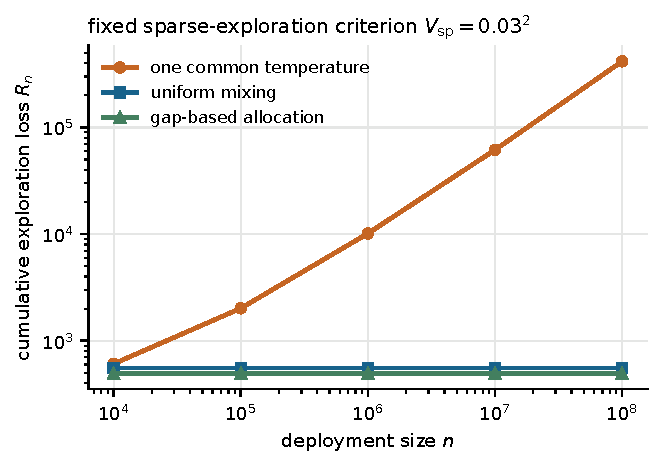
\includegraphics[width=0.55\textwidth]{figs/figA1_exploration_costs_small_delta.pdf}
\caption{As Figure~\ref{fig:costs}, with the sparse-exploration criterion fixed at
$V_{\rm sp}=0.03^2$.}
\label{fig:costs-small}
\end{figure}

\begin{figure}[tbp]
\centering
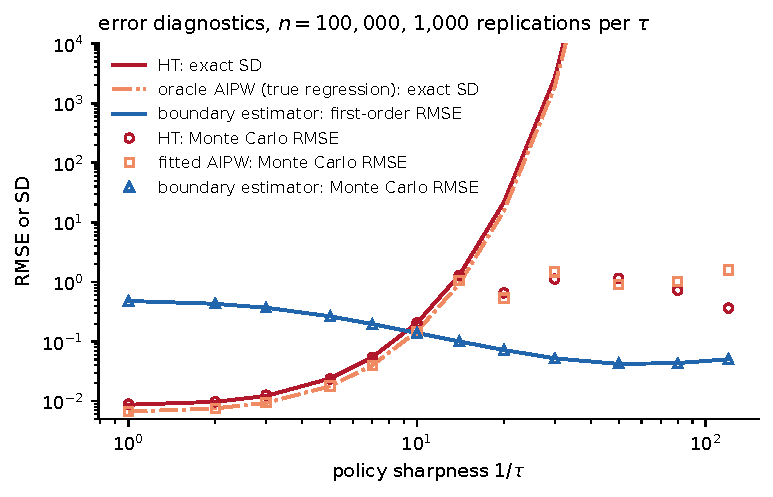
\includegraphics[width=0.7\textwidth]{figs/figA2_temperature_sweep_error.pdf}
\caption{Error diagnostics for the runs of Figure~\ref{fig:sweep}. Lines: exact
standard deviation of the Horvitz--Thompson estimator and of an oracle augmented
estimator that uses the true regression (a reference, not an estimator used in the
simulation), both for $\theta$, and the first-order approximation to the root mean
squared error of the boundary estimator of $\beta_0$. Markers: Monte Carlo root mean
squared error of the Horvitz--Thompson estimator, the augmented estimator with the
fitted working model, and the boundary estimator.}
\label{fig:sweep-error}
\end{figure}

\begin{table}[tbp]
\centering\small
\tabRD
\caption{Boundary effect $\beta_0=1$ at $n=10^5$, 1,000 replications, same logs for
both estimators: the estimator of Theorem~\ref{thm:boundary} (known probabilities)
and a fuzzy local-linear comparison at $\Delta=0$ (triangular kernel, bandwidth $b$,
heteroskedasticity-robust delta-method standard errors). ``Limit'' is the probability
limit, $\beta_{\ov,\tau}$ for the first estimator and the ratio of population
local-linear gaps for the second, computed by quadrature; ``first stage'' is the
population gap in the assignment probability. Very large errors reflect a small first
stage.}
\label{tab:rd}
\end{table}

\end{document}
